\section{Zielsetzung}
\label{sec:Zielsetzung}
Ziel des Versuches ist es die Bewegung der Leitungselektronen näher zu beschreiben. Dazu werden verschiedene mikroskopische Parameter aus den
zwei durchgeführten Versuchen berechnet.

\section{Theoretische Grundlage}
\label{sec:Theorie}

\subsection{Der Hall-Effekt}
Als Hall-Effekt wird das Auftreten einer Spannung in einem Stromdurchflossenen Leiter quer zur Richtung des Stroms bezeichnet, wenn sich der Leiter in einem äußeren Magnetfeld befindet. Die Spannung quer zur Stromrichtung lässt sich durch die Lorentz-Kraft erklären. In Abbildung \eqref{fig:Hall-Effekt} ist der  schematische Aufbau zur Beobachtung des Hall-Effektes zu sehen.

\begin{figure}[H]
	\centering
	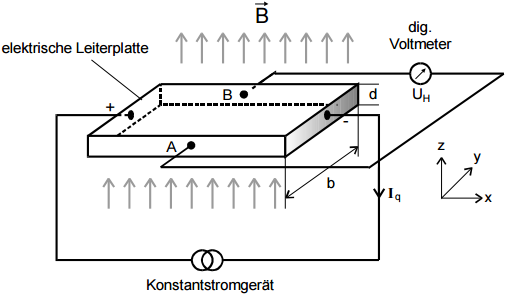
\includegraphics[height=7cm]{picture/Hall-Effekt.png}
	\caption{Schematischer Aufbau zur Beobachtung des Hall-Effektes. \cite[5]{sample}}
	\label{fig:Hall-Effekt}
\end{figure}

Im einfachsten Fall ist der Leiter ein Quader, weil die Breite $b$, die Länge $l$ und die Dicke $d$ sehr einfach gemessen werden können. Das Magnetfeld geht senkrecht durch die Fläche, welche von $b$ und $l$ aufgespannt wird. Der Strom fließt entlang der längsachse, wodurch auf die fließende Ladung die Lorentzkraft
\begin{equation}
	F_\text{L} = e_0\,\overline{v}_\text{D}\,B
	\label{eqn:FL}
\end{equation}
wirkt. Wobei $e_0$ für die Elementarladung, $v$ für die Geschwindigkeit der Elektronen und $B$ für die magnetische Flussdichte steht. Die Hall-Spannung $U_\text{H}$ lässt sich über das Kräftegleichgewicht zwischen Lorentz-Kraft und dem entstehenden elektrischen Feld bestimmen. Dazu wird noch $\overline{v}_\text{D}$ durch den Querstrom $I_\text{q}$ ausgedrückt.
\begin{equation}
	U_\text{H} = \frac{-1}{n\,e_0}\,\frac{B\,I_\text{q}}{d}
	\label{eqn:UH}
\end{equation}
Daraus kann die Ladungsträgerdichte $n$ bestimmt werden.


\subsection{Das Bändermodell von Kristallen}
Wenn eine Anzahl $m$ gleicher Atome dicht beieinander liegen, also einen Festkörper bilden, spalten sich deren Energieniveaus in je $m$ Zustände auf. Das äußerste Energienieveau kann dann nicht mehr für jedes Atom einzeln betrachtet werden, sondern muss dem Gesamtsystem zugeordnet werden. Allerdings liegen die Energieniveaus so dicht beieinander das sie als ein kontinuierliches Spektrum gesehen werden können, diese kontinuierlichen Spektren werden auch Bänder genannt. Die Bänder gehorchen dem Pauli-Prinzip, wodurch sich nur eine bestimmte Anzahl von Elektronen in einem Band aufhalten kann. Die Elektronen in den voll besetzten Bändern können ihr Energieniveau nicht verändern, das heißt sie können keine Energie aufnehmen oder abgeben. Zwischen den Bändern befinden sich verbotene Zonen, also Energiebereiche, die keine Zustände zulassen. In Abbildung \eqref{fig:Bandstruktur} ist das Bändermodell für Natrium aufgezeigt.

\begin{figure}[H]
	\centering
	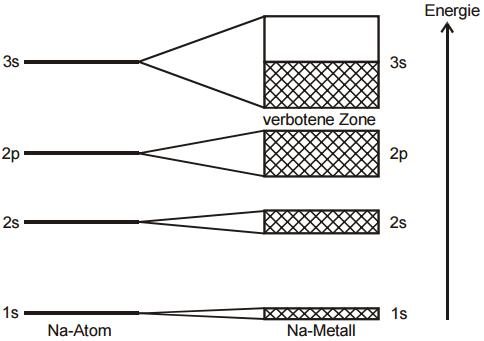
\includegraphics[height=7cm]{picture/Bandstruktur.png}
	\caption{Die Bandstruktur von Natrium. \cite[2]{sample}}
	\label{fig:Bandstruktur}
\end{figure}

In einem Leiter ist das oberste Band nur teilweise besetzt, wodurch die hohe Leitfähigkeit von Metallen hervorgerufen wird. Dieses Band wird Leitungsband genannt und die Elektronen darin werden Leitungselektronen genannt. Die Leitungselektronen bewegen sich in der Gitterstruktur wie die Teilchen eines idealen Gases. Es kann nun gezeigt werden, dass die Leitungselektronen nicht mit der Gitterstrukter eines idealen Kristalls wechselwirken, "da sich Materiewellen in einer streng periodischen Struktur ungehindert ausbreiten" \cite[2]{sample}. Daraus folgt das ein idealer Kristall keinen Widerstand besitzt, allerdings ist das praktisch nicht zu realisieren. Reale Proben sind nicht zu $100\,\%$ aus den selben Atomen gefertigt, auch ist die Gitterstruktur nicht exakt periodisch wodurch ein Widerstand entsteht. Außerdem kommt noch die Wärmebewegung der Ionenrümpfe hinzu wodurch die Ionen aus ihrer Gleichgewichtslage ausgelenkt werden und somit auch mit den Elektronen kollidieren können.


\subsection{Herleitung der elektrischen Leitfähigkeit eines Metalles}
Da sich die Leitungselektronen wie die Teilchen eines idealen Gases bewegen, stoßen sie mit den Fehlstellen des Gitters zusammen. Es kann nun über die Zeit zwischen zwei Zusammenstößen gemittelt werden. Daraus kann die mittlere Flugzeit $\overline{\tau}$ bestimmt werden. In der Zeit $\overline{\tau}$ führt das Elektron eine gleichmäßig beschleunigte Bewegung in die Richtung des elektrischen Feldes aus. Dadurch entsteht eine Geschwindigkeitsänderung $\Delta\overline{v}$ in Richtung des E-Feldes und daraus kann die mittlere Driftgeschwindigkeit $\overline{v}_\text{d}$ bestimmt werden.
\begin{equation}
	\overline{v}_\text{d} = \frac{\Delta\overline{v}}{2} = \frac{-\,e_0}{2\,m_0}\,\vec{E}\,\overline{\tau}
	\label{eqn:drift}
\end{equation}
Nun kann der elektrische Widerstand eines homogenen Leiters berechnet werden. Dafür wird die Stromdichte $j$ benötigt.
\begin{equation}
	j = -n\,\overline{v}_\text{d}\,e_0
	\label{eqn:j}
\end{equation}
Jetzt wird $j$ durch $\frac{I}{Q}$ ersetzt und $E$ durch $\frac{U}{L}$. \\
Aus diesen Überlegungen folgt der elektrische Widerstand $R$ zu
\begin{equation}
	R = \frac{2\,m_0\,L}{e_0^2\,n\,\overline{\tau}\,Q} \ .
	\label{eqn:R}
\end{equation}
$Q$ entspricht dabei dem Leiterquerschnitt, $L$ entspricht der Leiterlänge und $m_0$ ist die Masse eines Elektrons. \\
Aus dem elektrischen Widerstand kann nun noch der spezifische Widerstand $\rho$ hergeleitet werden.
\begin{equation}
	\rho = \frac{2\,m_0}{e_0^2\,n\,\overline{\tau}}
	\label{eqn:rho}
\end{equation}


\subsection{Herleitung weiterer mikroskopischer Leitfähigkeitsparameter}
Aus der Gleichung \eqref{eqn:j} kann die mittlere Driftgeschwindigkeit $\overline{v}_\text{d}$ errechnet werden, indem $j$ durch $I$ und $Q$ ersetzt wird. \\
Desweiteren kann die sogenannte mittlere freie Weglänge $\overline{l}$ bestimmt werden. Sie gibt die Entfernung zwischen zwei Zusammenstößen im Mittel an. Die mittlere freie Weglänge lässt sich aus
\begin{equation}
	\overline{l} = \overline{\tau}\,|v|
	\label{eqn:l}
\end{equation}
berechnen. "Hierin bedeutet $|v|$ die Totalgeschwindigkeit der Elektronen, die grundsätzlich von ihrer Driftgeschwindigkeit $\overline{v}_\text{d}$ verschieden ist" \cite[6]{sample}. Die Leitungselektronen unterliegen dem Pauli-Verbot, wodurch die Energieverteilung durch die Fermi-Dirac-Verteilung gegeben ist. Die Fermi-Dirac-Verteilung ist durch
\begin{equation}
	f(E)\,dE = \frac{1}{\exp\left(\frac{E - E_\text{F}}{k\,T}\right) + 1}\,dE
\end{equation}
gegeben. Wobei $E_\text{F}$ die Fermi-Dirac-Energie ist.
\begin{equation}
	E_\text{F} = \frac{h^2}{2\,m_0}\,\left(\frac{3\,n}{8\,\pi} \right)^{\frac{3}{2}}
\end{equation}
Daraus folgt für die mittlere freie Weglänge der Ausdruck
\begin{equation}
	\overline{l} = \overline{\tau}\,|\overline{v}| \approx \overline{\tau}\,\sqrt{\frac{2\,E_\text{F}}{m_0}} \ .
\end{equation}
Aus der mittleren Flugzeit $\overline{\tau}$ lässt sich die Beweglichkeit $\mu$ der Ladungsträger herleiten. Die Beweglichkeit ist definiert als Proportionalitätsfakor zwischen Driftgeschwindigkeit und der äußeren Feldstärke.
\begin{equation}
	\overline{v}_\text{d} = \mu\,E
	\label{eqn:Beweglichkeit}
\end{equation}
Die Anzahl der Ladungsträger pro Atom kann aus
\begin{equation}
	n_\text{A} = \frac{\Rho}{N\,U}
	\label{eqn:anzahl}
\end{equation}
berrechnet werden. Darin ist $\Rho$ die Dichte des Stoffs, $N$ ist die Anzahl der Atome und $U$ ist die Atomare Masseneinheit. 


\subsection{Elektrizitätsleistung in Metallen mit positiven Ladungsträgern}
Bei zweiwertigen Metallen kann es vorkommen, dass sich die Energiebänder überlappen. Dadurch können Elektronen von einem unteren Band in das angrezende darüberliegende Band übergehen. Im unteren Band entsteht dadurch eine Freistelle, welche als Loch bezeichnet wird. Diese Löcher bewegen sich unter dem Einfluss eines von außen anliegendem elektrischen Feld, und verhalten sich wie eine positive Ladung. Dieses Phänomen heißt anomaler Hall-Effekt. Dies ist bei der Messung durch ein umgekehrtes Vorzeichen der Hall-Spannung zu erkennen und es kann auf die Art der Ladungsträger geschlossen werden.






\subsection{Fehlerrechnung}
Sämtliche Fehlerrechnungen werden mit Hilfe von Python 3.4.3 durchgeführt.
\subsubsection{Mittelwert}
Der Mittelwert einer Messreihe $x_\text{1}, ... ,x_\text{n}$ lässt sich durch die Formel
\begin{equation}
	\overline{x} = \frac{1}{N} \sum_{\text{k}=1}^\text{N} x_k
	\label{eqn:ave}
\end{equation}
berechnen. Die Standardabweichung des Mittelwertes beträgt
\begin{equation}
	\Delta \overline{x} = \sqrt{ \frac{1}{N(N-1)} \sum_{\text{k}=1}^\text{N} (x_\text{k} - \overline{x})^2}
	\label{eqn:std}
\end{equation}

\subsubsection{Gauß'sche Fehlerfortpflanzung}
Wenn $x_\text{1}, ..., x_\text{n}$ fehlerbehaftete Messgrößen im weiteren Verlauf benutzt werden, wird der neue Fehler $\Delta f$ mit Hilfe der Gaußschen Fehlerfortpflanzung angegeben.
\begin{equation}
	\Delta f = \sqrt{\sum_{\text{k}=1}^\text{N} \left( \frac{ \partial f}{\partial x_\text{k}} \right) ^2 \cdot (\Delta x_\text{k})^2}
	\label{eqn:var}
\end{equation}

\subsubsection{Lineare Regression}
Die Steigung und y-Achsenabschnitt einer Ausgleichsgeraden werden gegebenfalls mittels Linearen Regression berechnet.
\begin{equation}
	y = m \cdot x + b
	\label{eqn:reg}
\end{equation}
\begin{equation}
	m = \frac{ \overline{xy} - \overline{x} \overline{y} } {\overline{x^2} - \overline{x}^2}
	\label{eqn:reg_m}
\end{equation}
\begin{equation}
	b = \frac{ \overline{x^2}\overline{y} - \overline{x} \, \overline{xy}} { \overline{x^2} - \overline{x}^2}
	\label{eqn:reg_b}
\end{equation}
